\documentclass{article}

% Sim2Science @ NeurIPS 2026 workshop camera-ready (de-anonymised).
\usepackage[dblblindworkshop, final]{neurips_2026}
\workshoptitle{Sim2Science: ML with Imperfect Scientific Models}

\usepackage[utf8]{inputenc}
\usepackage[T1]{fontenc}
\usepackage{hyperref}
\usepackage{url}
\usepackage{booktabs}
\usepackage{amsfonts}
\usepackage{amsmath,amssymb}
\usepackage{nicefrac}
\usepackage{microtype}
\usepackage{xcolor}
\usepackage{graphicx}
\graphicspath{{figures/}}

% Float separation tightened for the camera-ready page budget. Font, leading and margins
% are the neurips_2026 defaults and are not modified.
\setlength{\textfloatsep}{12pt plus 2pt minus 2pt}
\setlength{\floatsep}{10pt plus 2pt minus 2pt}
\setlength{\intextsep}{10pt plus 2pt minus 2pt}
\setlength{\abovecaptionskip}{6pt}
\setlength{\belowcaptionskip}{2pt}
% LaTeX's defaults reserve a fifth of any float-bearing page for text and cap how much of it a
% float may occupy, which left 14 blank lines and two underfull-vbox warnings on the page holding
% Fig. 1 and Table 1. Relaxing the fractions lets text and floats share those pages properly.
% Font size, leading and margins remain the neurips_2026 defaults.
\renewcommand{\topfraction}{0.95}
\renewcommand{\bottomfraction}{0.95}
\renewcommand{\textfraction}{0.06}
\renewcommand{\floatpagefraction}{0.85}

\title{Phantom Non-Identifiability:\\
When Simplifying a Coupled Simulator\\
Fabricates an Observability Boundary}

\author{%
  Ali Hariri Movahed\\
  RWTH Aachen University\\
  \texttt{ali.hariri.movahed@rwth-aachen.de}
}

\begin{document}
\maketitle

\begin{abstract}
Reduced simulators are the substrate of physics-informed surrogates and simulation-based inference,
and identifiability and optimal-sensor analyses are increasingly run on the same reduced model. We
show that a reduction severing the only path from a parameter to an observed field does not merely
lose accuracy: it manufactures a structural non-identifiability the real system does not have,
together with a confident prescription to buy an instrument the real system may not require for
identifiability. We demonstrate the mechanism on coupled heat and moisture (Luikov) transport, where
dropping the thermogradient (Posnov) coupling makes a Fisher analysis declare the moisture sensors
blind to the temperature-side parameters and an E-optimal step prescribe a temperature channel.
Restoring the term collapses the null: sensitivities grow as $O(\mathrm{Pn})$ and the Cram\'er-Rao
bound as $O(\mathrm{Pn}^{-1})$, which we derive and use to \emph{predict} the crossover from one probe
solve. Critically, the failure is silent -- over a wide window the calibrated reduced model passes a
$\chi^2$ goodness-of-fit test while still reporting rank $2$ and ``buy a temperature sensor'' -- and it
is not confined to inference: the same severed path zeros the input-to-observable Jacobian, so a
controller built on the reduced simulator pays up to $12.5\times$ the matched controller's closed-loop
cost while the objective component its own model treats as controllable improves. A frozen parametric
PINN inherits the phantom, and a two-head control rules out the obvious confound. We give the check
to run on other reductions.
\end{abstract}

\section{Introduction}
\paragraph{The mechanism.}\label{sec:intro-mech} A reduced simulator is safe for a task only if it preserves the directed
dependencies that task differentiates through. Inference and sensor design differentiate the
observation operator $H$ with respect to parameters $\theta$; control differentiates it with respect
to inputs $u$. \emph{Severing the only path from a parameter to an observable is
\textbf{sufficient} to create an exact null.} Neither converse holds: a surviving path may be weak,
wrong-signed or cancelling, and a severed one need not be fatal if the task's Jacobian is carried by
another route -- so the rule we draw is to check the relevant tangent map, not to audit path
structure.\footnote{``Observability'' here means local parameter identifiability (full column rank of the
scaled sensitivity, a finite Cram\'er-Rao bound) plus input-to-observable sensitivity, not classical
state observability or controllability.} Sever the only path and
$\partial H/\partial\theta_j\equiv0$ identically -- not small, zero -- so the reduced model reports
the parameter as structurally unidentifiable and an optimal-design step confidently prescribes new
instrumentation to repair a deficiency the system does not have.

Reductions of the same shape recur across multiphysics modelling, and we offer them as candidates
where the check below is worth running rather than as established instances: \emph{one-way coupling}
in fluid--structure interaction and particle-laden flow -- a phrase that sounds like a documented
approximation but is a structural claim about what can be inferred from what -- and likewise neglected
Soret or Dufour cross-diffusion, a zero Biot coefficient in poroelasticity, or frozen chemistry in a
reacting flow. Each severs a specific dependency.

\paragraph{This paper, and how we found it.} The system is coupled heat and moisture transport in a
drying sheet (the Luikov equations~\cite{luikov1975}), where a fast mesh-free surrogate is wanted as a
soft sensor for closed-loop control; PINNs~\cite{raissi2019} fit, and such systems are increasingly
modelled this way~\cite{manavi2024,laubscher2021}. Building one forces the identifiability question --
which parameters are recoverable from moisture-side sensors alone, and which extra instrument is
needed? -- now routinely posed on the same simplified simulator the surrogate is trained
on~\cite{cranmer2020sbi}. We built exactly that, and wrote it up: the parametric PINN on the reduced
($\mathrm{Pn}{=}0$) model, the Fisher analysis on it, the rank-2 null on
$\{\mathrm{Ko},\mathrm{Bi}_t\}$, and the E-optimal ``add a temperature channel'' prescription. A
pre-specified check of the dropped term, with thresholds fixed before the sweep was run, was meant to
confirm that result; it dissolved it. Sec.~\ref{sec:phantom} is the original analysis, unchanged;\footnote{Except that its temperature
channel is relabelled to the operator actually used, the mean $\langle T\rangle$; no result changed.} the
rest is the correction. We show the frozen PINN inheriting the phantom; by the same argument any
estimator trained only on the reduced simulator should inherit it, amortized SBI and neural operators
included, though we do not demonstrate those -- so a leaderboard-accurate surrogate can encode a
confident but wrong observability verdict, the misspecification regime this venue
targets~\cite{cranmer2020sbi}.

\paragraph{Related work.} Identifiability, Cram\'er-Rao bounds and optimal experimental design are
classical~\cite{kay1993,pukelsheim2006} and central to SBI under misspecification~\cite{cranmer2020sbi}.
For Luikov drying the inverse-problem literature poses estimation and design on \emph{temperature}
data -- by a D-optimum criterion over heat flux, timings and sensor placement~\cite{dantas2002}, on
the temperature field as sensitivity state variable~\cite{lugon2003}, or by a heat-flux profile making
all parameters simultaneously estimable~\cite{bensefia2011} -- and none asks what a
\emph{moisture-only} instrument can identify. Drying surrogates use PINNs on the reduced
model~\cite{raissi2019,manavi2024,laubscher2021}; discrepancy-corrected and universal PINNs learn
missing operators~\cite{zou2024misspecification,podina2023upinn} and derivative-informed surrogates
preserve high-fidelity Jacobians~\cite{olearyroseberry2024dino}, but these target state correction or
assume derivative labels. Closest are the literatures on model error itself: discrepancy-aware
Bayesian calibration, where ignoring discrepancy biases physical parameters and overstates
confidence~\cite{kennedy2001calibration,brynjarsdottir2014discrepancy}, and optimal design under
model error, irreducible~\cite{koval2020oed} or reducible~\cite{alexanderian2021oed}. All place the
discrepancy in the \emph{outputs}, leaving the tangent map intact; here the reduction zeros
$\partial H/\partial\theta_j$ exactly, which no output-space term can express, so the design verdict
flips while the fit stays good.

\paragraph{Contributions.} \textbf{(i)} The moisture-only null exists only at $\mathrm{Pn}{=}0$, and
we \emph{derive} rather than measure its dissolution. \textbf{(ii)} The failure is \emph{silent}: a
calibrated reduced model passes a $\chi^2$ goodness-of-fit test while returning the phantom null.
\textbf{(iii)} The sweep becomes a \emph{predictive} diagnostic from one probe solve, whose
distribution over the box we report by a Sobol design. \textbf{(iv)} A two-head control separates
inherited physics from a dead input, and no tested loss or architecture restores it. \textbf{(v)} The
same severed path removes the actuator's authority in closed loop. Throughout we validate the chain
end to end -- physical mass-flux operator, per-channel likelihood, Cram\'er-Rao against Monte Carlo, a
withheld instrument, and the joint five-parameter problem, which we report as \emph{not} well posed.
Code, the JSON artefact behind every number, and this paper's source:
\url{https://github.com/codebymov/phantom-non-identifiability}.

\section{Setup}\label{sec:setup}
\paragraph{Simulator.} On $\xi\in[0,1]$ (through-thickness, $\xi{=}0$ the hot-air surface) and
dimensionless time $\tau$, the Luikov system with the thermogradient coupling
is~\cite{lugon2003,luikov1975}
\begin{equation}\label{eq:luikov}
\partial_\tau T=\partial_{\xi\xi}T+\mathrm{Ko}\,\partial_\tau M,\qquad
\partial_\tau M=\mathrm{Lu}\,\partial_{\xi\xi}M+\underbrace{\mathrm{Lu}\,\mathrm{Pn}\,\partial_{\xi\xi}T}_{\text{thermogradient (Posnov)}},
\end{equation}
with Robin conditions at $\xi{=}0$ ($\partial_\xi T{=}\mathrm{Bi}_t(T{-}1)$, $\partial_\xi M{=}\mathrm{Bi}_m M$),
Neumann at $\xi{=}1$, and $T(\xi,0){=}0$, $M(\xi,0){=}1$. The standard reduction sets $\mathrm{Pn}{=}0$,
making the moisture balance autonomous; this is the form used across drying
surrogates~\cite{manavi2024,laubscher2021}. Ground truth is an implicit finite-difference (FD) solver
extended to carry $\mathrm{Pn}$ (default $0$, bit-identical to the reduced solver). The canonical
Luikov benchmark takes $\mathrm{Pn}{=}0.6$~\cite{lugon2003} and $[0.2,2]$ is the modelling range for
hygroscopic capillary-porous media~\cite{luikov1975}; assuming paper sits in that class, we call it
the \emph{assumed physical range} -- an assumption, not a measurement.

\paragraph{Observation operator.} A drying cell instruments two moisture quantities: a gravimetric
scale giving $\bar M(\tau)=\langle M(\cdot,\tau)\rangle_\xi$, and a mass-flow meter giving the surface
mass flux. In conservation form $\partial_\tau M=-\partial_\xi q_m$ with
$q_m=-\mathrm{Lu}(\partial_\xi M+\mathrm{Pn}\,\partial_\xi T)$, so the flux is the correct mass-flow
operator and, with the Neumann back boundary, $q_m(0,\tau)=\mathrm{d}\bar M/\mathrm{d}\tau$ exactly.
The Robin conditions give both boundary derivatives in closed form, so no numerical differentiation
enters:
\begin{equation}\label{eq:flux}
q_m(0,\tau)=-\mathrm{Lu}\bigl(\mathrm{Bi}_m M(0,\tau)+\mathrm{Pn}\,\mathrm{Bi}_t(T(0,\tau)-1)\bigr).
\end{equation}
They remain separate instruments with independent noise; stacked over $K{=}40$ sample times they form
$H_M$, with $\langle T\rangle{=}\langle T(\cdot,\tau)\rangle_\xi$ the optional addition -- used for the
gain row of Table~\ref{tab:pn} and the E-optimal step of Sec.~\ref{sec:phantom}, while
App.~\ref{app:valid} withholds the surface trace $T(0,\tau)$. On the grid used the identity holds
discretely to $0.4\%$ for $\mathrm{Pn}\!\le\!0.2$, degrading to $2.6\%$ at $\mathrm{Pn}{=}2$ as the
explicit thermogradient term grows; it doubles as a conservation check.

\paragraph{Noise model and identifiability.} Each channel carries independent Gaussian noise with
$\sigma_c$ equal to $1\%$ of its own range. We form the scaled sensitivity $S_{ij}=\partial H_i/\partial\log\theta_j$ for
$\theta=(\mathrm{Lu},\mathrm{Ko},\mathrm{Bi}_t,\mathrm{Bi}_m)$ by central differences through the
solver ($d{=}10^{-3}$ in $\log\theta$), the Fisher information $F=S^\top\Sigma^{-1}S$, and the Cram\'er-Rao (CR) relative standard
deviation~\cite{kay1993}. Because $\mathrm{Ko}$ and $\mathrm{Bi}_t$ enter only the temperature
equation, \emph{at $\mathrm{Pn}{=}0$ the moisture balance is autonomous and Eq.~\ref{eq:flux}
collapses to $-\mathrm{Lu}\,\mathrm{Bi}_m M(0,\tau)$, so
$\partial H_M/\partial\mathrm{Ko}=\partial H_M/\partial\mathrm{Bi}_t\equiv 0$, $\mathrm{rank}(S)=2$,
and one mean-temperature channel restores full column rank.} That one-line fact is the whole of the
reduced-model result; the contribution is what happens when the dropped term returns. Rank is read from the
scaled columns, not an eigenvalue ratio -- column $j$ counts when
$\|S_{:j}/\sigma\|>10^{-9}\max_k\|S_{:k}/\sigma\|$ -- so weak-but-nonzero coupling is reported by the
CR bound, never as a spurious null.

\section{What the reduced simulator prescribes ($\mathrm{Pn}{=}0$)}\label{sec:phantom}
At the nominal $\theta{=}(0.5,2,1,1)$ the moisture-only $\{\mathrm{Ko},\mathrm{Bi}_t\}$ sensitivity
columns are exactly zero and $\mathrm{rank}(S)=2$. On the reduced model this reads as a firm design
law: an E-optimal ($\lambda_{\min}(F)$) selection~\cite{pukelsheim2006} lifts $\lambda_{\min}$ from
$0$ to $3.2{\times}10^{2}$ by adding a mean-temperature channel, matching the temperature-first
prescription of the Luikov literature~\cite{dantas2002,bensefia2011}. The reduced simulator hands the
experimenter a confident
verdict: moisture instrumentation is structurally insufficient. Three estimators agree, the misfit
being exactly flat in those coordinates: solver-in-the-loop least squares and an amortized estimator
fitting the $(\mathrm{Ko},\mathrm{Bi}_t)$ inputs of a frozen parametric PINN never leave their
\emph{initialisation}, and ensemble-Kalman inversion~\cite{iglesias2013eki} -- the only one with a
prior in the Bayesian sense -- does not contract. The surrogate's architecture, training budget and
forward accuracy are in App.~\ref{app:surrogate}.

\paragraph{Control: inherited physics, or a dead input?}\label{par:control} A vanishing derivative with
respect to a network input is equally the signature of a coordinate never learned, so the inheritance
claim and a training failure are indistinguishable as usually stated. They separate without
retraining, because the same network has two heads and $\mathrm{Ko}$ reaches them by different routes:
directly in the temperature equation, and into the moisture equation \emph{only} through the dropped
term. Autograd through the frozen surrogate gives
$\|\partial\langle T\rangle/\partial\log\mathrm{Ko}\|=2.498$ against the solver's $2.485$ ($1.2\%$)
while $\|\partial\langle M\rangle/\partial\log\mathrm{Ko}\|=0.022$ against its exact zero
($\mathrm{Bi}_t$ behaves the same). A dead input would zero both heads. One caveat: the moisture-head
residue is not exactly zero, and at roughly $7\%$ of the true coupled sensitivity at the best-converged
arm (App.~\ref{app:e1}) it is small but not negligible -- a surrogate's tangent map can report a
coupling as small, and cannot certify it as zero. Nor is it an objective one can fix: gradient-enhanced penalties,
gradient-norm balancing, causal weighting and a shared trunk feeding $T$ and $\partial_\xi T$ straight
to the moisture head all drive the severed sensitivity \emph{toward} zero rather than toward its true
coupled value, over three seeds; the architecture built to let the pathway reappear is
indistinguishable from objectives with no such design (App.~\ref{app:e1}).

\section{The boundary dissolves, and the rate is derivable}\label{sec:dissolve}
The reduction is not free: the full moisture balance carries the thermogradient term
$\mathrm{Lu}\,\mathrm{Pn}\,\partial_{\xi\xi}T$~\cite{lugon2003}. Expanding about the decoupled
solution, $M=M_0+\mathrm{Pn}\,M_1+O(\mathrm{Pn}^2)$ with
$\partial_\tau M_1=\mathrm{Lu}\,\partial_{\xi\xi}M_1+\mathrm{Lu}\,\partial_{\xi\xi}T_0$, both channels
inherit $\mathrm{Ko},\mathrm{Bi}_t$ only through $T_0$ at first order (the flux also through the
explicit $\mathrm{Pn}\,\mathrm{Bi}_t$ term of Eq.~\ref{eq:flux}, likewise $O(\mathrm{Pn})$). Hence
\begin{equation}\label{eq:scaling}
\partial H_M/\partial\log\theta_j=\mathrm{Pn}\,a_j(\theta)+O(\mathrm{Pn}^2),\qquad
F_{jj}=\mathrm{Pn}^2a_j^2/\sigma^2,\qquad
\mathrm{CR}(\theta_j)=\gamma_j(\theta)/\mathrm{Pn}+O(1).
\end{equation}
Over $\mathrm{Pn}\in[10^{-3},10^{-1}]$ the log-log slopes of the two CR bounds are $-0.959$ and
$-0.990$ against $-1$ from Eq.~\ref{eq:scaling}, and the CR falls through the $100\%$ usability line
at a derived rather than measured rate (Fig.~\ref{fig:cross}a, Table~\ref{tab:pn}). Two statements
must be kept apart. \emph{Analytically}, Eq.~\ref{eq:scaling} removes the exact null wherever
$a_j(\theta)\neq0$ -- the generic case, since $T_0$ carries $\mathrm{Ko}$ and $\mathrm{Bi}_t$ and the
restored $\mathrm{Lu}\,\mathrm{Pn}\,\partial_{\xi\xi}T_0$ is not identically zero -- but does not
exclude isolated $\theta$ where some $a_j$ vanishes. \emph{Numerically}, $\mathrm{rank}(S){=}4$ at
every tested $\mathrm{Pn}{>}0$, over the box and the $K{=}40$ schedule. Identifiability is graded, not binary, in three regimes: exactly zero columns at
$\mathrm{Pn}{=}0$; nonzero but nearly parallel to the $\{\mathrm{Lu},\mathrm{Bi}_m\}$ columns for
$0<\mathrm{Pn}\!\lesssim\!0.7$ ($|\mathrm{corr}(\mathrm{Ko},\mathrm{Bi}_t)|{=}0.997$ at
$\mathrm{Pn}{=}0.2$), where the marginal CR stays large through collinearity rather than a null; and
genuinely separated above $\mathrm{Pn}\!\approx\!0.8$, where those correlations collapse and the
marginal CR falls steeply (Fig.~\ref{fig:cross}a).

\paragraph{A predictive diagnostic, not a sweep.} Eq.~\ref{eq:scaling} makes the crossover
$\mathrm{Pn}^\star$ (where $\mathrm{CR}=100\%$) equal to $\gamma_j(\theta)$, which one probe solve
estimates as $\mathrm{CR}(\theta_j;\mathrm{Pn}_{\text{probe}})\cdot\mathrm{Pn}_{\text{probe}}$.
Against bisection over the $16$ box corners this is accurate to $4.5\%$ median and $15.5\%$ max where
the crossover is itself weakly coupled ($\mathrm{Pn}^\star\!<\!0.05$), degrading to $18.7\%$ median
where $\mathrm{Pn}^\star=O(1)$ -- a failure the probe itself flags. Comparing $\mathrm{Pn}^\star$ with
the plausible range of the dropped coefficient is the operational test: below that range the null is a
phantom, above it the reduced model's verdict stands. The test settles the \emph{structural} claim --
identifiability in principle -- not whether the instrument is worth buying. It presumes the dropped
term is known and restorable with a plausible range, and $\mathrm{Pn}^\star$ inherits the $100\%$
threshold, noise model, schedule and nuisance choice: a check for a \emph{suspected} coupling, not a
detector of unknown structural error.

\paragraph{Crossover distribution.} Over $256$ Sobol points the crossover has median
$\mathrm{Pn}^\star{=}0.037$ (interquartile $[0.019,0.089]$), and $88\%$ of the box lies below $0.2$, the bottom of the assumed physical range: for most operating
conditions $\{\mathrm{Ko},\mathrm{Bi}_t\}$ cross the $100\%$ CR line at realistic coupling
\emph{with $\mathrm{Pn}$ known} -- identifiability in principle, not precision, since below
$\mathrm{Pn}\!\approx\!1$ they stay weakly determined (App.~\ref{app:valid}). The remaining $12\%$
(low $\mathrm{Lu}$ and $\mathrm{Ko}$) never crosses it.

\begin{figure}[!htbp]\centering
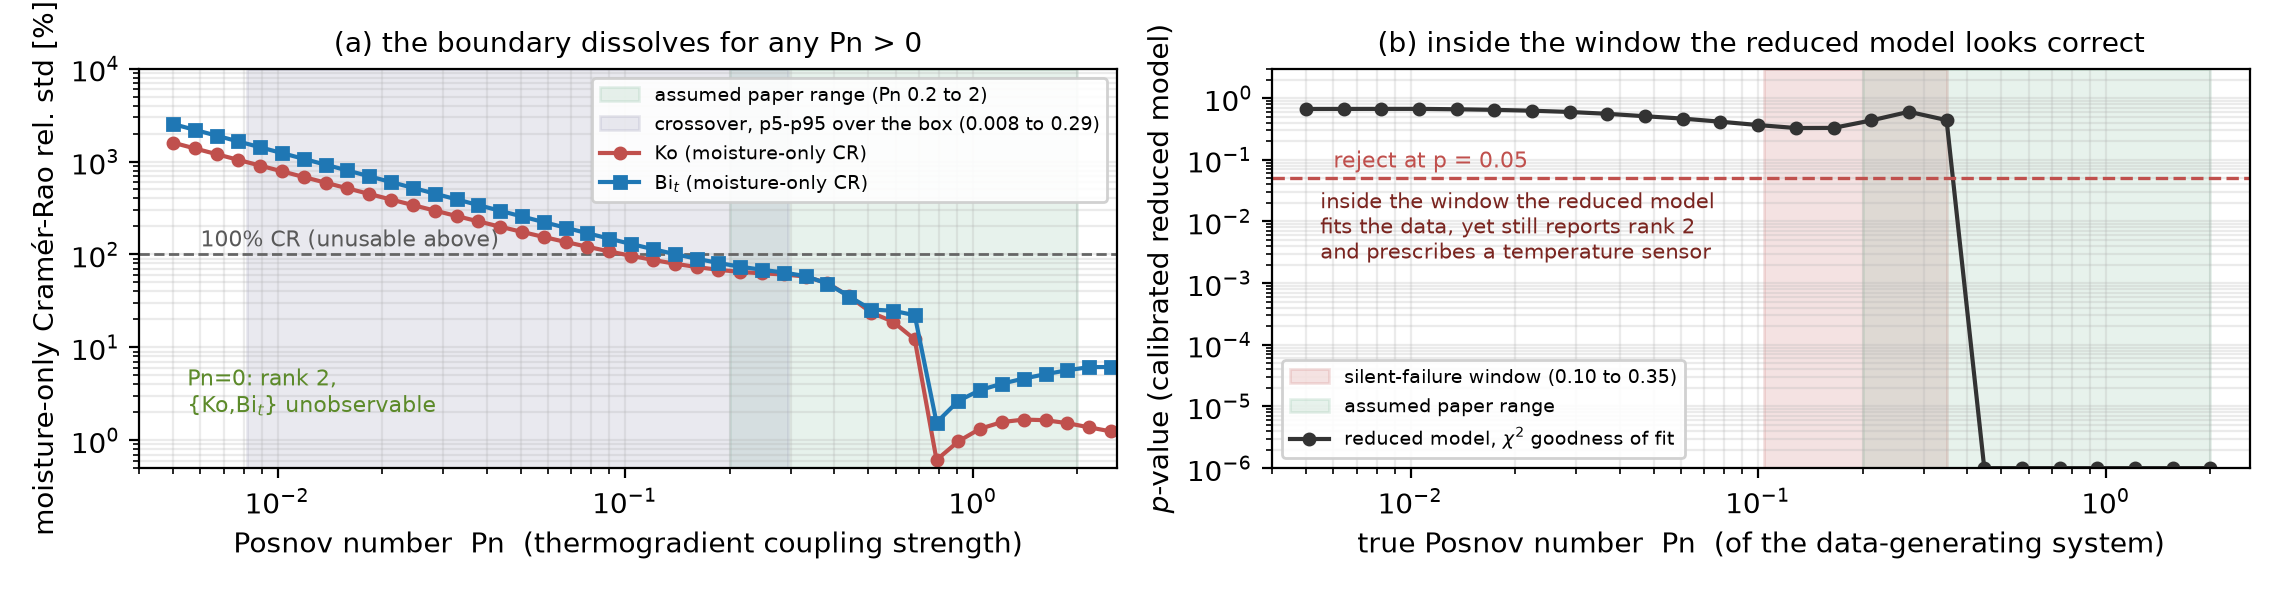
\includegraphics[width=.72\linewidth]{P_posnov_crossover.png}
\caption{\textbf{(a)} Moisture-only CR relative std for $\{\mathrm{Ko},\mathrm{Bi}_t\}$ vs.\ the
Posnov coupling: unidentifiable at $\mathrm{Pn}{=}0$, full rank at every tested $\mathrm{Pn}{>}0$.
\textbf{(b)} The failure is silent: the reduced model, calibrated over
$(\mathrm{Lu},\mathrm{Bi}_m)$ against the same noisy moisture data, passes a $\chi^2$ test up to
$\mathrm{Pn}{=}0.35$ while returning the phantom null throughout. Between the crossover ($0.0996$ at
the nominal $\theta$) and the top of that band, nothing signals that anything is wrong.}
\label{fig:cross}
\end{figure}

\begin{table}[!htbp]\centering\small
\caption{Moisture-only identifiability vs.\ Posnov number (nominal $\theta$, $K{=}40$, per-channel
noise $1\%$ of range). Gain is the moisture-only to moisture-plus-$\langle T\rangle$ CR ratio;
$\mathrm{rank}(S){=}2$ at $\mathrm{Pn}{=}0$, $4$ at every tested $\mathrm{Pn}{>}0$.}
\label{tab:pn}
\begin{tabular}{lcccccc}\toprule
$\mathrm{Pn}$ & $0.0$ & $0.05$ & $0.1$ & $0.2$ & $0.6$ & $1.0$\\\midrule
CR $\mathrm{Ko}$ & $\infty$ & $176\%$ & $99\%$ & $66\%$ & $19\%$ & $1.2\%$\\
CR $\mathrm{Bi}_t$ & $\infty$ & $259\%$ & $134\%$ & $77\%$ & $26\%$ & $3.2\%$\\\midrule
gain from a $T$ channel ($\mathrm{Ko}$) & $\infty$ & $34\times$ & $14\times$ & $5.1\times$ & $8.1\times$ & $1.2\times$\\
\bottomrule\end{tabular}

\end{table}

\section{The failure is silent}\label{sec:silent}
At $\mathrm{Pn}{=}0.6$ the reduced model at the true parameters leaves a $17\%$ moisture
discrepancy, which would be caught before its verdict was trusted. But a practitioner calibrates
first, and calibration launders the misspecification into the parameters it \emph{can} see. We generate noisy moisture-only observations from the
full model at each true $\mathrm{Pn}$, fit $(\mathrm{Lu},\mathrm{Bi}_m)$ under the reduced model in
the operating box, and test the residual against the known per-channel noise ($\chi^2$, $20$ seeds,
$2K{-}2$ d.o.f.). It passes at $\alpha{=}0.05$ up to $\mathrm{Pn}{=}0.35$ (Fig.~\ref{fig:cross}b),
where the median $p$-value is $0.44$ and the calibrated discrepancy $0.2\%$, down from $11.9\%$ --
the error absorbed as bias in $\mathrm{Lu}$, pulled from $0.5$ to $0.33$, while the Jacobian rotates
and the sensitivity ordering inverts (App.~\ref{app:valid}). Throughout, the reduced model reports $\mathrm{rank}(S)=2$, $\mathrm{CR}=\infty$ and ``buy a temperature sensor''.
The window runs from $\mathrm{Pn}^\star{=}0.0996$ to $0.35$, overlapping the assumed range on
$[0.2,0.35]$: goodness of fit misses the problem because the misspecification is invisible in the
observables and lethal only in the Jacobian.

\section{OSSE: recovery, robustness, and the joint problem}\label{sec:osse}
The Fisher verdict is estimator-agnostic; we confirm it with an estimator. From the two noisy
moisture-only channels we recover the ``unobservable'' pair by solver-in-the-loop least squares in
log-parameter space, from a wrong initialisation, under either forward model
(Table~\ref{tab:osse}). Under the reduced model the estimator is frozen with zero variance across
seeds and at every noise level from $0.2\%$ to $5\%$: the misfit is exactly flat, so the pair is
\emph{structurally impossible} to recover. Under the full model the \emph{same} channels recover
both to $0.1\%$ (Table~\ref{tab:osse}). Under a genuine instrument
misspecification (unmodelled $3\%$ gain, $0.5\%$ bias) $\mathrm{Ko}$ degrades to $12.7\%$, which the
temperature channel only improves to $9.6\%$.

\paragraph{Validation, and the limit of the claim.} The Cram\'er-Rao bound agrees with the
estimator's Monte Carlo spread once compared like with like, and a moisture-only fit predicts a
withheld surface-temperature channel the reduced model cannot (App.~\ref{app:valid}). But local full
rank is not global identifiability: a five-parameter recovery from random initialisations leaves
$\mathrm{Bi}_t,\mathrm{Bi}_m$ at $45\%$ and $41\%$, in more than one basin. The dissolution concerns
the $\{\mathrm{Ko},\mathrm{Bi}_t\}$ null, not the well-posedness of the joint problem: with
$\mathrm{Pn}$ known that is unimodal but well determined only at the strongest coupling we tested,
$\mathrm{Pn}{=}1$ (App.~\ref{app:valid}).

\section{Implications, mitigation, and conclusion}\label{sec:impl}
\paragraph{Inheritance and a model-uncertain correction.} Estimators trained on the reduced
simulator cannot recover a parameter it made invisible, whatever their forward accuracy. Fixing
$\mathrm{Pn}{=}0$ is the degenerate structural prior $p(\mathrm{Pn}){=}\delta_0$; a spike-and-slab
instead returns uncertainty over $J=\partial H/\partial\theta$ and the sensor ranking, and tracks the
matched controller for $\mathrm{Pn}\!\ge\!0.35$, at a cost where the coupling is weak
(App.~\ref{app:control}). What we invalidate is the \emph{structural} argument -- that moisture
instrumentation is categorically insufficient -- not the instrument: under $\mathrm{Pn}$ uncertainty
a temperature channel still informs $\mathrm{Pn}$, breaks the collinearity and cuts the bound at
every tested $\mathrm{Pn}{>}0$ (Table~\ref{tab:pn}). Nor is fitting observations enough, the object
that must be right being the tangent map: a discrepancy network should learn a conservative
cross-field \emph{flux} with parameter--discrepancy separation~\cite{plumlee2018orthogonal},
checkable by our two-head control and set out as a three-step audit in App.~\ref{app:procedure}.

\paragraph{Phantom uncontrollability.} The severed path corrupts intervention as well as inference.
With the hot-air temperature $u$ manipulated, the reduced plant advances moisture by an operator
referencing neither $u$ nor $T$: $\partial\bar M/\partial u\equiv0$ to machine precision while the
actuator keeps full authority over temperature, returning at first order like the parameter Jacobian.
The consequence is a decision, not a bound: at $\mathrm{Pn}{=}0.35$, inside the silent band, a
reduced-model controller pays $8\times$ the matched controller's cost while the component its own
model treats as controllable improves (App.~\ref{app:control}).

\paragraph{Limitations and the lesson.} All results are in silico from one solver family and one
coupled system; a second system and output feedback are future work. The Posnov range is assumed.
The silent band uses one noise model, schedule and box, with its $\chi^2$ test on the calibration
data and the two fitted parameters removed from the d.o.f. The lesson: validating a reduced
simulator's \emph{outputs} is insufficient when inference or control depends on tangent maps it has
severed.

\begin{ack}
The question was suggested by the Institut f\"ur Textiltechnik (ITA) of RWTH Aachen University, and
I thank Flemming Heuvel for the discussions that shaped it. All modelling, implementation,
experiments and analysis reported here are my own.
\end{ack}

{\small\bibliographystyle{plain}\bibliography{references}}

\newpage
\section*{NeurIPS Paper Checklist}




\begin{enumerate}

\item {\bf Claims}
    \item[] Question: Do the main claims made in the abstract and introduction accurately reflect the paper's contributions and scope?
    \item[] Answer: \answerYes{} % Replace by \answerYes{}, \answerNo{}, or \answerNA{}.
    \item[] Justification: The abstract and Sec.~\ref{sec:intro-mech} claims -- the exact rank-2 null at $\mathrm{Pn}{=}0$, its $O(\mathrm{Pn})$ dissolution, the silent goodness-of-fit band, the one-probe crossover prediction, the two-head surrogate control, and the corrected sensor-design conclusion (the reduced model's categorical ``moisture sensing is structurally insufficient'' verdict is false under the coupled model over the assumed $\mathrm{Pn}$ range; we do not claim a temperature channel is unnecessary) -- are each supported by a correspondingly numbered result in Secs.~3--7.
    \item[] Guidelines:
    \begin{itemize}
        \item The answer \answerNA{} means that the abstract and introduction do not include the claims made in the paper.
        \item The abstract and/or introduction should clearly state the claims made, including the contributions made in the paper and important assumptions and limitations. A \answerNo{} or \answerNA{} answer to this question will not be perceived well by the reviewers. 
        \item The claims made should match theoretical and experimental results, and reflect how much the results can be expected to generalize to other settings. 
        \item It is fine to include aspirational goals as motivation as long as it is clear that these goals are not attained by the paper. 
    \end{itemize}

\item {\bf Limitations}
    \item[] Question: Does the paper discuss the limitations of the work performed by the authors?
    \item[] Answer: \answerYes{} % Replace by \answerYes{}, \answerNo{}, or \answerNA{}.
    \item[] Justification: Sec.~\ref{sec:impl} (Limitations) states that all results are in silico from one solver family and one coupled system; that a second physical system, and output-feedback control in place of the full-state feedback we use, are future work; that the Posnov range is assumed rather than measured for a paper grade; that the silent band is measured under a single noise model, schedule and parameter box, with its $\chi^2$ test evaluated on the calibration data and the two fitted parameters removed from the d.o.f.; and App.~\ref{app:e1} states that its arms all train on reduced physics, so it confirms the analytic claim rather than benchmarking mitigations. Sec.~\ref{sec:osse} additionally reports that the joint five-parameter inverse problem is \emph{not} well posed, and Sec.~\ref{sec:dissolve} that identifiability below the collinearity collapse is limited by collinearity rather than by a null.
    \item[] Guidelines:
    \begin{itemize}
        \item The answer \answerNA{} means that the paper has no limitation while the answer \answerNo{} means that the paper has limitations, but those are not discussed in the paper. 
        \item The authors are encouraged to create a separate ``Limitations'' section in their paper.
        \item The paper should point out any strong assumptions and how robust the results are to violations of these assumptions (e.g., independence assumptions, noiseless settings, model well-specification, asymptotic approximations only holding locally). The authors should reflect on how these assumptions might be violated in practice and what the implications would be.
        \item The authors should reflect on the scope of the claims made, e.g., if the approach was only tested on a few datasets or with a few runs. In general, empirical results often depend on implicit assumptions, which should be articulated.
        \item The authors should reflect on the factors that influence the performance of the approach. For example, a facial recognition algorithm may perform poorly when image resolution is low or images are taken in low lighting. Or a speech-to-text system might not be used reliably to provide closed captions for online lectures because it fails to handle technical jargon.
        \item The authors should discuss the computational efficiency of the proposed algorithms and how they scale with dataset size.
        \item If applicable, the authors should discuss possible limitations of their approach to address problems of privacy and fairness.
        \item While the authors might fear that complete honesty about limitations might be used by reviewers as grounds for rejection, a worse outcome might be that reviewers discover limitations that aren't acknowledged in the paper. The authors should use their best judgment and recognize that individual actions in favor of transparency play an important role in developing norms that preserve the integrity of the community. Reviewers will be specifically instructed to not penalize honesty concerning limitations.
    \end{itemize}

\item {\bf Theory assumptions and proofs}
    \item[] Question: For each theoretical result, does the paper provide the full set of assumptions and a complete (and correct) proof?
    \item[] Answer: \answerYes{} % Replace by \answerYes{}, \answerNo{}, or \answerNA{}.
    \item[] Justification: The structural claim (Sec.~\ref{sec:setup}) is a one-line consequence of the moisture balance being autonomous at $\mathrm{Pn}{=}0$, with its assumptions stated alongside it and verified numerically (columns exactly zero, $\mathrm{rank}(S){=}2$). The scaling law (Eq.~\ref{eq:scaling}) is a first-order expansion about the decoupled solution, valid for $\mathrm{Pn}\ll1$; its predicted exponents are checked against measurement ($-0.959$, $-0.990$ vs $-1$) and its predictive use is reported separately inside and outside its regime of validity. Sec.~\ref{sec:dissolve} separates what the expansion proves -- no exact null wherever $a_j(\theta)\neq0$, which does not exclude isolated $\theta$ at which some $a_j$ vanishes -- from the numerical finding of full rank at every \emph{tested} $\mathrm{Pn}{>}0$ over the box and the $K{=}40$ schedule, and Sec.~\ref{sec:setup} states the scaled-column-norm criterion by which rank is decided.
    \item[] Guidelines:
    \begin{itemize}
        \item The answer \answerNA{} means that the paper does not include theoretical results. 
        \item All the theorems, formulas, and proofs in the paper should be numbered and cross-referenced.
        \item All assumptions should be clearly stated or referenced in the statement of any theorems.
        \item The proofs can either appear in the main paper or the supplemental material, but if they appear in the supplemental material, the authors are encouraged to provide a short proof sketch to provide intuition. 
        \item Inversely, any informal proof provided in the core of the paper should be complemented by formal proofs provided in appendix or supplemental material.
        \item Theorems and Lemmas that the proof relies upon should be properly referenced. 
    \end{itemize}

    \item {\bf Experimental result reproducibility}
    \item[] Question: Does the paper fully disclose all the information needed to reproduce the main experimental results of the paper to the extent that it affects the main claims and/or conclusions of the paper (regardless of whether the code and data are provided or not)?
    \item[] Answer: \answerYes{} % Replace by \answerYes{}, \answerNo{}, or \answerNA{}.
    \item[] Justification: Governing equations (Eq.~\ref{eq:luikov}), the flux observation operator (Eq.~\ref{eq:flux}), the finite-difference discretisation, the sensor and noise model, seeds, grids, sample count $K$, and all thresholds are stated in-text. Every experiment imports one shared observation model, so the Fisher analysis and the estimator experiments cannot diverge.
    \item[] Guidelines:
    \begin{itemize}
        \item The answer \answerNA{} means that the paper does not include experiments.
        \item If the paper includes experiments, a \answerNo{} answer to this question will not be perceived well by the reviewers: Making the paper reproducible is important, regardless of whether the code and data are provided or not.
        \item If the contribution is a dataset and\slash or model, the authors should describe the steps taken to make their results reproducible or verifiable. 
        \item Depending on the contribution, reproducibility can be accomplished in various ways. For example, if the contribution is a novel architecture, describing the architecture fully might suffice, or if the contribution is a specific model and empirical evaluation, it may be necessary to either make it possible for others to replicate the model with the same dataset, or provide access to the model. In general. releasing code and data is often one good way to accomplish this, but reproducibility can also be provided via detailed instructions for how to replicate the results, access to a hosted model (e.g., in the case of a large language model), releasing of a model checkpoint, or other means that are appropriate to the research performed.
        \item While NeurIPS does not require releasing code, the conference does require all submissions to provide some reasonable avenue for reproducibility, which may depend on the nature of the contribution. For example
        \begin{enumerate}
            \item If the contribution is primarily a new algorithm, the paper should make it clear how to reproduce that algorithm.
            \item If the contribution is primarily a new model architecture, the paper should describe the architecture clearly and fully.
            \item If the contribution is a new model (e.g., a large language model), then there should either be a way to access this model for reproducing the results or a way to reproduce the model (e.g., with an open-source dataset or instructions for how to construct the dataset).
            \item We recognize that reproducibility may be tricky in some cases, in which case authors are welcome to describe the particular way they provide for reproducibility. In the case of closed-source models, it may be that access to the model is limited in some way (e.g., to registered users), but it should be possible for other researchers to have some path to reproducing or verifying the results.
        \end{enumerate}
    \end{itemize}


\item {\bf Open access to data and code}
    \item[] Question: Does the paper provide open access to the data and code, with sufficient instructions to faithfully reproduce the main experimental results, as described in supplemental material?
    \item[] Answer: \answerYes{} % Replace by \answerYes{}, \answerNo{}, or \answerNA{}.
    \item[] Justification: All code and artefacts are public under an MIT licence at \url{https://github.com/codebymov/phantom-non-identifiability}, including the finite-difference solver, every analysis script, the JSON artefact behind every reported number, and this paper's LaTeX source. The repository README maps each table, figure and inline value to the script that produces it and the artefact key that stores it. No external datasets are used; all data are simulated, so the repository is self-contained and runs on a laptop CPU. The paper additionally states everything needed to reimplement from scratch: the governing equations (Eq.~\ref{eq:luikov}), the conservation-form observation operator (Eq.~\ref{eq:flux}), the discretisation, the per-channel noise model, seeds, grids, sample count $K$, the central-difference step, the surrogate architecture and training budget (App.~\ref{app:surrogate}), and the control objective with all weights, bounds and solver settings (Eq.~\ref{eq:mpc}, App.~\ref{app:control}).
    \item[] Guidelines:
    \begin{itemize}
        \item The answer \answerNA{} means that paper does not include experiments requiring code.
        \item Please see the NeurIPS code and data submission guidelines (\url{https://neurips.cc/public/guides/CodeSubmissionPolicy}) for more details.
        \item While we encourage the release of code and data, we understand that this might not be possible, so \answerNo{} is an acceptable answer. Papers cannot be rejected simply for not including code, unless this is central to the contribution (e.g., for a new open-source benchmark).
        \item The instructions should contain the exact command and environment needed to run to reproduce the results. See the NeurIPS code and data submission guidelines (\url{https://neurips.cc/public/guides/CodeSubmissionPolicy}) for more details.
        \item The authors should provide instructions on data access and preparation, including how to access the raw data, preprocessed data, intermediate data, and generated data, etc.
        \item The authors should provide scripts to reproduce all experimental results for the new proposed method and baselines. If only a subset of experiments are reproducible, they should state which ones are omitted from the script and why.
        \item At submission time, to preserve anonymity, the authors should release anonymized versions (if applicable).
        \item Providing as much information as possible in supplemental material (appended to the paper) is recommended, but including URLs to data and code is permitted.
    \end{itemize}


\item {\bf Experimental setting/details}
    \item[] Question: Does the paper specify all the training and test details (e.g., data splits, hyperparameters, how they were chosen, type of optimizer) necessary to understand the results?
    \item[] Answer: \answerYes{} % Replace by \answerYes{}, \answerNo{}, or \answerNA{}.
    \item[] Justification: Sec.~\ref{sec:setup} gives the observation operator, noise model and central-difference step; App.~\ref{app:surrogate} gives the surrogate's architecture (two MLPs, width 96, depth 6, hard initial conditions), its training budget (8000 collocation points, 12k Adam then 1.5k L-BFGS) and its forward accuracy; Sec.~\ref{sec:osse} gives the estimator (Levenberg--Marquardt in log-parameter space from a stated wrong initialisation); Sec.~\ref{sec:setup} gives the central-difference step ($d{=}10^{-3}$ in $\log\theta$); and App.~\ref{app:control} gives the control study's objective, cost weights, horizon, control interval, input bounds and optimiser.
    \item[] Guidelines:
    \begin{itemize}
        \item The answer \answerNA{} means that the paper does not include experiments.
        \item The experimental setting should be presented in the core of the paper to a level of detail that is necessary to appreciate the results and make sense of them.
        \item The full details can be provided either with the code, in appendix, or as supplemental material.
    \end{itemize}

\item {\bf Experiment statistical significance}
    \item[] Question: Does the paper report error bars suitably and correctly defined or other appropriate information about the statistical significance of the experiments?
    \item[] Answer: \answerYes{} % Replace by \answerYes{}, \answerNo{}, or \answerNA{}.
    \item[] Justification: Recovery experiments use 20 seeds and report mean $\pm$ standard deviation; the noise level is swept from $0.2\%$ to $5\%$ of range; the goodness-of-fit test reports the fraction of seeds passing at $\alpha{=}0.05$; the joint inverse problems use multi-start and report medians -- the four-parameter study at known $\mathrm{Pn}$ (Table~\ref{tab:joint4}) over $20$ seeds $\times$ $4$ random starts from the box at each of three noise levels, reporting per-parameter medians, the fraction of starts reaching the best basin and the fraction of seeds recovering all four parameters to $10\%$; and the loss and architecture study (App.~\ref{app:e1}) reports mean $\pm$ s.d.\ over three seeds. The closed-loop study uses four multistarts per solve, against which no reported cost moves by more than $0.05\%$. Cram\'er-Rao bounds are additionally cross-checked against the Monte Carlo spread.
    \item[] Guidelines:
    \begin{itemize}
        \item The answer \answerNA{} means that the paper does not include experiments.
        \item The authors should answer \answerYes{} if the results are accompanied by error bars, confidence intervals, or statistical significance tests, at least for the experiments that support the main claims of the paper.
        \item The factors of variability that the error bars are capturing should be clearly stated (for example, train/test split, initialization, random drawing of some parameter, or overall run with given experimental conditions).
        \item The method for calculating the error bars should be explained (closed form formula, call to a library function, bootstrap, etc.)
        \item The assumptions made should be given (e.g., Normally distributed errors).
        \item It should be clear whether the error bar is the standard deviation or the standard error of the mean.
        \item It is OK to report 1-sigma error bars, but one should state it. The authors should preferably report a 2-sigma error bar than state that they have a 96\% CI, if the hypothesis of Normality of errors is not verified.
        \item For asymmetric distributions, the authors should be careful not to show in tables or figures symmetric error bars that would yield results that are out of range (e.g., negative error rates).
        \item If error bars are reported in tables or plots, the authors should explain in the text how they were calculated and reference the corresponding figures or tables in the text.
    \end{itemize}

\item {\bf Experiments compute resources}
    \item[] Question: For each experiment, does the paper provide sufficient information on the computer resources (type of compute workers, memory, time of execution) needed to reproduce the experiments?
    \item[] Answer: \answerYes{} % Replace by \answerYes{}, \answerNo{}, or \answerNA{}.
    \item[] Justification: All experiments run on a laptop CPU in minutes. One finite-difference solve is a few milliseconds; the one-probe diagnostic is a few dozen solves; the largest sweep is a few hundred thousand solves.
    \item[] Guidelines:
    \begin{itemize}
        \item The answer \answerNA{} means that the paper does not include experiments.
        \item The paper should indicate the type of compute workers CPU or GPU, internal cluster, or cloud provider, including relevant memory and storage.
        \item The paper should provide the amount of compute required for each of the individual experimental runs as well as estimate the total compute. 
        \item The paper should disclose whether the full research project required more compute than the experiments reported in the paper (e.g., preliminary or failed experiments that didn't make it into the paper). 
    \end{itemize}
    
\item {\bf Code of ethics}
    \item[] Question: Does the research conducted in the paper conform, in every respect, with the NeurIPS Code of Ethics \url{https://neurips.cc/public/EthicsGuidelines}?
    \item[] Answer: \answerYes{} % Replace by \answerYes{}, \answerNo{}, or \answerNA{}.
    \item[] Justification: The research conforms to the NeurIPS Code of Ethics. It is a simulation study with no human subjects, no personal data, and no released models with foreseeable misuse potential.
    \item[] Guidelines:
    \begin{itemize}
        \item The answer \answerNA{} means that the authors have not reviewed the NeurIPS Code of Ethics.
        \item If the authors answer \answerNo, they should explain the special circumstances that require a deviation from the Code of Ethics.
        \item The authors should make sure to preserve anonymity (e.g., if there is a special consideration due to laws or regulations in their jurisdiction).
    \end{itemize}


\item {\bf Broader impacts}
    \item[] Question: Does the paper discuss both potential positive societal impacts and negative societal impacts of the work performed?
    \item[] Answer: \answerYes{} % Replace by \answerYes{}, \answerNo{}, or \answerNA{}.
    \item[] Justification: Discussed in Sec.~\ref{sec:impl} and below: better drying soft sensors can reduce industrial energy use, and the paper's caution is that identifiability and sensor-design verdicts computed on reduced simulators can misdirect instrumentation investment. We see no negative societal impact specific to this work.
    \item[] Guidelines:
    \begin{itemize}
        \item The answer \answerNA{} means that there is no societal impact of the work performed.
        \item If the authors answer \answerNA{} or \answerNo, they should explain why their work has no societal impact or why the paper does not address societal impact.
        \item Examples of negative societal impacts include potential malicious or unintended uses (e.g., disinformation, generating fake profiles, surveillance), fairness considerations (e.g., deployment of technologies that could make decisions that unfairly impact specific groups), privacy considerations, and security considerations.
        \item The conference expects that many papers will be foundational research and not tied to particular applications, let alone deployments. However, if there is a direct path to any negative applications, the authors should point it out. For example, it is legitimate to point out that an improvement in the quality of generative models could be used to generate Deepfakes for disinformation. On the other hand, it is not needed to point out that a generic algorithm for optimizing neural networks could enable people to train models that generate Deepfakes faster.
        \item The authors should consider possible harms that could arise when the technology is being used as intended and functioning correctly, harms that could arise when the technology is being used as intended but gives incorrect results, and harms following from (intentional or unintentional) misuse of the technology.
        \item If there are negative societal impacts, the authors could also discuss possible mitigation strategies (e.g., gated release of models, providing defenses in addition to attacks, mechanisms for monitoring misuse, mechanisms to monitor how a system learns from feedback over time, improving the efficiency and accessibility of ML).
    \end{itemize}
    
\item {\bf Safeguards}
    \item[] Question: Does the paper describe safeguards that have been put in place for responsible release of data or models that have a high risk for misuse (e.g., pre-trained language models, image generators, or scraped datasets)?
    \item[] Answer: \answerNA{} % Replace by \answerYes{}, \answerNo{}, or \answerNA{}.
    \item[] Justification: The paper releases analysis code for a physical simulation study. It releases no pretrained generative models, scraped datasets, or other artefacts carrying a risk of misuse.
    \item[] Guidelines:
    \begin{itemize}
        \item The answer \answerNA{} means that the paper poses no such risks.
        \item Released models that have a high risk for misuse or dual-use should be released with necessary safeguards to allow for controlled use of the model, for example by requiring that users adhere to usage guidelines or restrictions to access the model or implementing safety filters. 
        \item Datasets that have been scraped from the Internet could pose safety risks. The authors should describe how they avoided releasing unsafe images.
        \item We recognize that providing effective safeguards is challenging, and many papers do not require this, but we encourage authors to take this into account and make a best faith effort.
    \end{itemize}

\item {\bf Licenses for existing assets}
    \item[] Question: Are the creators or original owners of assets (e.g., code, data, models), used in the paper, properly credited and are the license and terms of use explicitly mentioned and properly respected?
    \item[] Answer: \answerYes{} % Replace by \answerYes{}, \answerNo{}, or \answerNA{}.
    \item[] Justification: The work uses only standard open-source scientific libraries (NumPy, SciPy, PyTorch, Matplotlib) under their permissive licences, and the official NeurIPS 2026 style files. No third-party datasets or pretrained models are used. Prior work whose results or formulations we build on is cited in-text.
    \item[] Guidelines:
    \begin{itemize}
        \item The answer \answerNA{} means that the paper does not use existing assets.
        \item The authors should cite the original paper that produced the code package or dataset.
        \item The authors should state which version of the asset is used and, if possible, include a URL.
        \item The name of the license (e.g., CC-BY 4.0) should be included for each asset.
        \item For scraped data from a particular source (e.g., website), the copyright and terms of service of that source should be provided.
        \item If assets are released, the license, copyright information, and terms of use in the package should be provided. For popular datasets, \url{paperswithcode.com/datasets} has curated licenses for some datasets. Their licensing guide can help determine the license of a dataset.
        \item For existing datasets that are re-packaged, both the original license and the license of the derived asset (if it has changed) should be provided.
        \item If this information is not available online, the authors are encouraged to reach out to the asset's creators.
    \end{itemize}

\item {\bf New assets}
    \item[] Question: Are new assets introduced in the paper well documented and is the documentation provided alongside the assets?
    \item[] Answer: \answerYes{} % Replace by \answerYes{}, \answerNo{}, or \answerNA{}.
    \item[] Justification: The code and artefacts released at \url{https://github.com/codebymov/phantom-non-identifiability} are documented: an MIT licence, a README giving install steps, runtime tiers and the number-to-script-to-artefact map, and per-script docstrings stating each script's purpose, method, assumptions and invocation. Known limitations of the implementation are recorded there too. No dataset, model checkpoint or trained artefact is released, only source and the JSON results.
    \item[] Guidelines:
    \begin{itemize}
        \item The answer \answerNA{} means that the paper does not release new assets.
        \item Researchers should communicate the details of the dataset\slash code\slash model as part of their submissions via structured templates. This includes details about training, license, limitations, etc. 
        \item The paper should discuss whether and how consent was obtained from people whose asset is used.
        \item At submission time, remember to anonymize your assets (if applicable). You can either create an anonymized URL or include an anonymized zip file.
    \end{itemize}

\item {\bf Crowdsourcing and research with human subjects}
    \item[] Question: For crowdsourcing experiments and research with human subjects, does the paper include the full text of instructions given to participants and screenshots, if applicable, as well as details about compensation (if any)? 
    \item[] Answer: \answerNA{} % Replace by \answerYes{}, \answerNo{}, or \answerNA{}.
    \item[] Justification: The paper involves no crowdsourcing and no research with human subjects.
    \item[] Guidelines:
    \begin{itemize}
        \item The answer \answerNA{} means that the paper does not involve crowdsourcing nor research with human subjects.
        \item Including this information in the supplemental material is fine, but if the main contribution of the paper involves human subjects, then as much detail as possible should be included in the main paper. 
        \item According to the NeurIPS Code of Ethics, workers involved in data collection, curation, or other labor should be paid at least the minimum wage in the country of the data collector. 
    \end{itemize}

\item {\bf Institutional review board (IRB) approvals or equivalent for research with human subjects}
    \item[] Question: Does the paper describe potential risks incurred by study participants, whether such risks were disclosed to the subjects, and whether Institutional Review Board (IRB) approvals (or an equivalent approval/review based on the requirements of your country or institution) were obtained?
    \item[] Answer: \answerNA{} % Replace by \answerYes{}, \answerNo{}, or \answerNA{}.
    \item[] Justification: The paper involves no research with human subjects, so no IRB review was required.
    \item[] Guidelines:
    \begin{itemize}
        \item The answer \answerNA{} means that the paper does not involve crowdsourcing nor research with human subjects.
        \item Depending on the country in which research is conducted, IRB approval (or equivalent) may be required for any human subjects research. If you obtained IRB approval, you should clearly state this in the paper. 
        \item We recognize that the procedures for this may vary significantly between institutions and locations, and we expect authors to adhere to the NeurIPS Code of Ethics and the guidelines for their institution. 
        \item For initial submissions, do not include any information that would break anonymity (if applicable), such as the institution conducting the review.
    \end{itemize}

\item {\bf Declaration of LLM usage}
    \item[] Question: Does the paper describe the usage of LLMs if it is an important, original, or non-standard component of the core methods in this research? Note that if the LLM is used only for writing, editing, or formatting purposes and does \emph{not} impact the core methodology, scientific rigor, or originality of the research, declaration is not required.
    %this research? 
    \item[] Answer: \answerNA{} % Replace by \answerYes{}, \answerNo{}, or \answerNA{}.
    \item[] Justification: LLMs are not a component of the core methodology. The methods are a finite-difference Luikov solver, Fisher-information and Cram\'er-Rao analysis, a physics-trained parametric surrogate, and solver-in-the-loop nonlinear model-predictive control. LLM assistance was limited to writing and coding support, which the stated policy does not require to be declared.
    \item[] Guidelines:
    \begin{itemize}
        \item The answer \answerNA{} means that the core method development in this research does not involve LLMs as any important, original, or non-standard components.
        \item Please refer to our LLM policy in the NeurIPS handbook for what should or should not be described.
    \end{itemize}

\end{enumerate}

\appendix
\section{Surrogate details}\label{app:surrogate}
The amortized estimator of Sec.~\ref{sec:phantom} fits the $(\mathrm{Ko},\mathrm{Bi}_t)$ inputs of a
frozen parametric PINN: two MLPs (width $96$, depth $6$, hard-enforced initial conditions) over
$(\xi,\tau,\mathrm{Bi}_t,\mathrm{Bi}_m,\mathrm{Lu},\mathrm{Ko})$, trained physics-only on $8000$
collocation points for $12$k Adam then $1.5$k L-BFGS iterations. Forward accuracy at the nominal
point is rel-$L_2$ $0.012$ on $\langle M\rangle$ and $0.111$ on $\langle T\rangle$. The temperature
head's field error being $11\%$ while its $\mathrm{Ko}$-sensitivity matches the solver to $1.2\%$ is
not a contradiction: a network can misplace a field's level and still capture how that field responds
to a parameter, and it is the latter that the two-head control of Sec.~\ref{sec:phantom} relies on to
establish that the zero moisture-side sensitivity is inherited physics rather than a training
artefact.

\section{Validation detail}\label{app:valid}
\begin{table}[!htbp]\centering\small
\caption{OSSE recovery of the ``unobservable'' pair from the two moisture channels (truth
$\mathrm{Pn}{=}0.6$, $\theta^\star{=}(0.5,2,1,1)$; initialisation $\mathrm{Ko}{=}1,\mathrm{Bi}_t{=}0.5$;
20 seeds, $1\%$ noise). The reduced model is frozen on every grid and at every noise level.}
\label{tab:osse}
\begin{tabular}{llcc}\toprule
forward model & truth / instrument & $\mathrm{Ko}$ (true $2.0$) & $\mathrm{Bi}_t$ (true $1.0$)\\\midrule
\textbf{full} ($\mathrm{Pn}{=}0.6$) & matched grid & $2.00\!\pm\!0.01$ (\textbf{0.1\%}) & $1.00\!\pm\!0.00$ (\textbf{0.0\%})\\
\textbf{reduced} ($\mathrm{Pn}{=}0$) & matched grid & $1.00\!\pm\!0.00$ (frozen) & $0.50\!\pm\!0.00$ (frozen)\\
full ($\mathrm{Pn}{=}0.6$) & $4\times$ refined grid & $2.01\!\pm\!0.01$ ($0.6\%$) & $1.00\!\pm\!0.00$ ($0.1\%$)\\
full ($\mathrm{Pn}{=}0.6$) & gain/bias error & $1.75\!\pm\!0.01$ ($12.7\%$) & $0.98\!\pm\!0.00$ ($2.2\%$)\\
\bottomrule\end{tabular}
\end{table}

\textbf{Cram\'er-Rao against Monte Carlo.} Table~\ref{tab:pn} reports $19.2\%$ on $\mathrm{Ko}$ where
Table~\ref{tab:osse} recovers it to $0.1\%$. These agree: the former is the \emph{marginal} bound with
$\mathrm{Lu},\mathrm{Bi}_m$ also unknown, while the estimator holds them fixed. The comparable
\emph{conditional} bound is $0.4\%$ against a Monte Carlo spread of $0.37\%$, which is what validates
the Fisher machinery the rest of the paper rests on.

\textbf{Where the calibration error goes.} At the top of the silent band the misfit is absorbed as
bias in the parameters the reduced model can see: $\mathrm{Lu}$ is pulled from $0.5$ to $0.33$, the
Jacobian's sensitive subspace rotates by $68^\circ$, and the sensitivity ordering inverts -- so the
calibrated model is wrong in a way no residual reveals.

\textbf{A withheld instrument.} Predicting a channel never fitted separates physical recovery from
compensation within the moisture channels. From the moisture-only fit the full model reproduces the
surface-temperature trace $T(0,\tau)$ to $0.0\%$ on a matched grid and $2.1\%$ under the instrument
misspecification of Table~\ref{tab:osse}; the reduced model, frozen at its initialisation, misses it
by $48.9\%$.

\textbf{The observation operator deserves equal scrutiny.} Writing the mass-flow meter as
$\partial_\tau M(0,\tau)$ rather than the conservation-form flux of Eq.~\ref{eq:flux} leaves the null
untouched but inflates apparent discretisation error by two orders of magnitude. Relatedly, the gain
row of Table~\ref{tab:pn} is non-monotonic because it is a ratio of two bounds improving at different
rates: the collinearity collapse near $\mathrm{Pn}\!\approx\!0.8$ helps the moisture-only set far more
than the already well-conditioned moisture-plus-$\langle T\rangle$ set.

\textbf{The joint problem with the coupling known.} App.~\ref{app:procedure}'s audit ends with the
dropped coefficient measured, so the practical case is the four-parameter problem at \emph{known}
$\mathrm{Pn}$. Recovering $(\mathrm{Lu},\mathrm{Ko},\mathrm{Bi}_t,\mathrm{Bi}_m)$ from the two
moisture channels under the full model, with Table~\ref{tab:osse}'s estimator and $4$ random starts
from the box per seed ($20$ seeds), \emph{every} start reaches the same basin in every cell of
Table~\ref{tab:joint4}: the multimodality of the five-parameter problem below comes from estimating
$\mathrm{Pn}$ itself, not from the coupled model. Accuracy, though, is strongly graded in
$\mathrm{Pn}$ and tracks the marginal CR of Table~\ref{tab:pn}. At $\mathrm{Pn}{=}1$ all four recover
to a few per cent; at the canonical $\mathrm{Pn}{=}0.6$ benchmark $\mathrm{Ko}$ and $\mathrm{Bi}_t$
reach only $13\%$ and $20\%$; at $\mathrm{Pn}{=}0.2$ they are not usefully determined ($36\%$,
$48\%$). Every median estimate is interior to the box, so this is the collinearity of
Sec.~\ref{sec:dissolve} rather than a boundary artefact. Dissolving the null is therefore not a claim
that the moisture-only cell pins down the whole parameter vector: it does so only at
$\mathrm{Pn}{=}1$, the strongest coupling we tested, which is the other half of the scoping in
Sec.~\ref{sec:impl}. The assumed range runs to $\mathrm{Pn}{=}2$, which we did not test.

\begin{table}[h]\centering\footnotesize
\setlength{\tabcolsep}{5pt}
\caption{Joint recovery of all four parameters from the two moisture channels with $\mathrm{Pn}$
known and fixed (full model, $20$ seeds $\times$ $4$ random starts from the box, best-cost start per
seed). Median relative error per parameter; ``all four'' is the fraction of seeds within $10\%$ on
every parameter simultaneously. Every start reached the same basin in every row.}
\label{tab:joint4}
\begin{tabular}{ccccccc}\toprule
$\mathrm{Pn}$ & noise & $\mathrm{Lu}$ & $\mathrm{Ko}$ & $\mathrm{Bi}_t$ & $\mathrm{Bi}_m$ & all four\\\midrule
$0.2$ & $0.5\%$ & $2.5\%$ & $24.9\%$ & $28.1\%$ & $4.2\%$ & $15\%$\\
$0.2$ & $1\%$   & $4.8\%$ & $35.8\%$ & $47.6\%$ & $5.0\%$ & $10\%$\\
$0.2$ & $2\%$   & $8.0\%$ & $39.9\%$ & $50.0\%$ & $8.3\%$ & $5\%$\\\midrule
$0.6$ & $0.5\%$ & $11.7\%$ & $9.5\%$ & $13.7\%$ & $12.6\%$ & $40\%$\\
$0.6$ & $1\%$   & $17.0\%$ & $13.2\%$ & $19.7\%$ & $18.7\%$ & $25\%$\\
$0.6$ & $2\%$   & $31.0\%$ & $16.9\%$ & $45.2\%$ & $39.8\%$ & $15\%$\\\midrule
$1.0$ & $0.5\%$ & $1.4\%$ & $0.5\%$ & $1.0\%$ & $0.9\%$ & $100\%$\\
$1.0$ & $1\%$   & $2.8\%$ & $1.1\%$ & $2.0\%$ & $1.8\%$ & $100\%$\\
$1.0$ & $2\%$   & $5.5\%$ & $2.2\%$ & $3.9\%$ & $3.6\%$ & $90\%$\\
\bottomrule\end{tabular}
\end{table}

\textbf{The joint problem with the coupling unknown.} Recovering all five of
$(\mathrm{Lu},\mathrm{Ko},\mathrm{Bi}_t,\mathrm{Bi}_m,\mathrm{Pn})$ from random initialisations across
the box, the coupling is best determined ($\mathrm{Pn}$ to $1.8\%$ median) and $\mathrm{Ko}$ reaches
$18\%$, but $\mathrm{Bi}_t$ and $\mathrm{Bi}_m$ land at $45\%$ and $41\%$ and the multi-start residual
costs reveal more than one basin.

\section{Tested loss and architecture modifications do not restore the severed pathway}\label{app:e1}
If the residual is built from the reduced operator, $\mathrm{Ko}$ and $\mathrm{Bi}_t$ appear only in
the temperature equation and the moisture balance is autonomous. Differentiating that residual with
respect to $\mathrm{Ko}$ shows the sensitivity $\partial M/\partial\mathrm{Ko}$ obeys the same
homogeneous equation with homogeneous initial and boundary data, so its unique solution is zero: the
null is a property of the hypothesis space, not of the objective, and a loss can only reweight paths
that already exist. A trained network realises this only up to its own residual error, so what is
measured is a \emph{leakage floor} rather than an exact zero.

This appendix exists to confirm that analytic claim on a finitely-trained network, not to benchmark
mitigations: every arm trains on the reduced operator, so every arm is \emph{expected} to fail, and
an arm doing better here would mean its optimisation left less residue, not that it recovered the
severed physics. Data from the coupled system, or an embedded discrepancy term, would reintroduce
the missing pathway and is the actual fix -- that is the point of the mitigation in
Sec.~\ref{sec:impl} -- and is out of scope here by construction.

We test it against the remedies a PINN-literate reader would reach for. Five arms train on the same
reduced physics with the same budget ($12$k Adam then $800$ L-BFGS steps, width $96$, depth $5$,
$4000$ collocation points, three seeds) and differ only in objective or architecture; the last is
deliberately the most favourable case, a shared trunk whose moisture head receives the temperature
head's output and its spatial gradient as explicit inputs.

\begin{table}[h]\centering\footnotesize
\setlength{\tabcolsep}{4pt}
\caption{None of the tested objectives or architectures restores the severed pathway. All arms train on the \emph{same} reduced ($\mathrm{Pn}{=}0$) physics and differ only in objective or architecture; mean $\pm$ s.d.\ over 3 seeds. The solver's reduced-model value for $\|\partial\langle M\rangle/\partial\log\mathrm{Ko}\|$ is exactly $0$; under the true model ($\mathrm{Pn}{=}0.6$) it is $0.372$. ``Leakage'' is the severed-pathway sensitivity as a fraction of the intact $\mathrm{Ko}\!\to\!\langle T\rangle$ pathway of the same network, given in the preceding column. $\dagger$: one of the three baseline seeds does not converge (per-seed leakage $1.8$, $7.3$, $137.5\%$), so its mean would not summarise a stable quantity and its denominator is itself unreliable; the median is given instead.}
\label{tab:e1}
\begin{tabular}{lccccc}\toprule
arm & fwd rel-$L_2$ & $\|\partial_{\log\mathrm{Ko}}\langle M\rangle\|$ & $\|\partial_{\log\mathrm{Ko}}\langle T\rangle\|$ & leakage & vs.\ true\\\midrule
baseline residual & $0.066\pm0.072$ & $0.233\pm0.202$ & $1.52$ & $7.3\%^\dagger$ & $63\%$\\
$+$ gradient-enhanced penalty & $0.008\pm0.004$ & $0.121\pm0.075$ & $2.16$ & $5.8\pm3.8\%$ & $32\%$\\
$+$ gradient-norm balancing & $0.008\pm0.003$ & $0.027\pm0.018$ & $2.33$ & $1.1\pm0.7\%$ & $7\%$\\
$+$ causal weighting & $0.013\pm0.005$ & $0.115\pm0.064$ & $2.09$ & $5.7\pm3.4\%$ & $31\%$\\
shared trunk, $T$ and $\partial_\xi T$ to the $M$ head & $0.010\pm0.002$ & $0.123\pm0.049$ & $2.14$ & $5.9\pm2.5\%$ & $33\%$\\
\bottomrule\end{tabular}
\end{table}


\paragraph{Reading.} The structural claim is the analytical one above, and it is exact: at convergence
the reduced residual forces $\partial\langle M\rangle/\partial\mathrm{Ko}$ to zero, so no objective can
reintroduce the pathway. The table reports what a \emph{finitely}-trained network does with that, over
three seeds.

Three things follow. First, leakage is optimisation residue, not a structural quantity: the plain
baseline is unstable across seeds ($1.8$, $7.3$, $137.5\%$; one run fails to converge, so
Table~\ref{tab:e1} gives its median), while every modification that stabilises training also drives
leakage down, gradient-norm balancing furthest ($1.1\pm0.7\%$). Second, and the point of the experiment, \emph{none} of them moves the severed
sensitivity toward the true coupled value; they move it toward zero, which is the correct answer under
the reduced physics. Third, the architecture built to let the pathway reappear buys nothing: the shared
trunk, which receives $T$ and $\partial_\xi T$ as explicit inputs, sits at $5.9\pm2.5\%$ against
$5.8\pm3.8\%$ for a gradient-enhanced penalty and $5.7\pm3.4\%$ for causal weighting -- indistinguishable
from modifications with no such design, and beaten by pure loss balancing. The practical consequence is
why the diagnostic of Sec.~\ref{sec:dissolve} runs on the solver and not the surrogate: even at the best
arm the residue is $7\%$ of the true coupled sensitivity, so a surrogate's tangent map can report a
coupling \emph{small} but cannot certify it \emph{zero}. The loss column is omitted as it is not
comparable across arms, the adaptive arm reweighting the boundary term by construction.

\section{A three-step audit for a candidate reduction}\label{app:procedure}
The mitigation of Sec.~\ref{sec:impl} is a procedure, and this is it. It is cheap: every step below
is a solver call, and the whole audit for our system runs in minutes on a laptop CPU.

\textbf{1. Enumerate what the reduction dropped, and what it severs.} For each term the reduced
model omits, write down which directed paths it removes from the observation operator
$H(\theta)$ \emph{and} from $H(u)$ -- the two differ, and a reduction safe for inference can still
be fatal for control, as $\mathrm{Pn}{=}0$ is here. For the Luikov reduction, dropping
$\mathrm{Lu}\,\mathrm{Pn}\,\partial_{\xi\xi}T$ severs the only path from $\{\mathrm{Ko},\mathrm{Bi}_t\}$
to the moisture channels, and the only path from $u$ to $\bar M$.

\textbf{2. Probe the crossover at the bottom of each plausible range.} Restore the term in the
simulator, run one probe solve at a small coefficient value, and read off
$\mathrm{Pn}^\star\!\approx\!\mathrm{CR}(\theta_j;\mathrm{Pn}_{\text{probe}})\cdot\mathrm{Pn}_{\text{probe}}$
(Sec.~\ref{sec:dissolve}), with its stated assumptions. Comparing $\mathrm{Pn}^\star$ against the
\emph{lower} end of the coefficient's plausible range is the conservative test.

\textbf{3. Act on the comparison.} If $\mathrm{Pn}^\star$ falls inside the plausible range, the
reduced model's verdict is a phantom and must not be used for identifiability or sensor design:
replace the implicit $p(\mathrm{Pn}){=}\delta_0$ with a spike-and-slab prior, measure or estimate the
coefficient, and re-run the design analysis on the coupled model. If $\mathrm{Pn}^\star$ sits above
the whole range, the reduced verdict stands on the evidence available. If the range straddles
$\mathrm{Pn}^\star$, report the verdict as range-dependent rather than resolved -- and note that
goodness of fit will not settle it, since the silent band of Sec.~\ref{sec:silent} overlaps exactly
this region.

\section{Phantom uncontrollability: closed-loop detail}\label{app:control}
The control plant of our repository takes the hot-air temperature $u$ as the manipulated variable and
advances moisture with an operator that references neither $u$ nor $T$ -- the $\mathrm{Pn}{=}0$
reduction. Its docstring nonetheless asserts that higher air temperature dries faster, which the
implementation makes impossible: the control-side instance of this paper's thesis, authored by us. Its input-to-moisture Jacobian is therefore exactly zero, not merely small
(Fig.~\ref{fig:ctrl}a), while the actuator retains full authority over surface temperature
($\|\partial T(0,\tau)/\partial u\|=9.0$). Restoring
the coupling recovers drying authority at first order, with measured log-log slopes $+0.994$
($\bar M$) and $+0.995$ (drying rate) for $\mathrm{Pn}\!\le\!0.1$ -- the same law the
parameter-to-observation Jacobian obeys.

\paragraph{Task, objective and arms.} Reach a terminal mean-moisture target while holding the surface
at a quality setpoint below a scorching limit. Raising $u$ helps the temperature term and hurts the
moisture term, a trade-off that exists only for $\mathrm{Pn}>0$. The shrinking-horizon cost is
\begin{equation}\label{eq:mpc}
J=q_T\!\sum_k (T_k-T_{\text{set}})^2\Delta\tau
+q_M (\bar M_N-\bar M_{\text{target}})^2
+r\!\sum_b (\Delta u_b)^2
+\rho\!\sum_k \bigl[T_k-T_{\text{crit}}\bigr]_+^2\Delta\tau ,
\end{equation}
with $T_{\text{set}}{=}0.55$, $T_{\text{crit}}{=}0.65$, $\bar M_{\text{target}}{=}0.565$,
$q_T{=}1$, $q_M{=}400$, $r{=}0.05$, $\rho{=}200$; plant step $\Delta\tau{=}0.01$ over
$\tau\in(0,2]$, a control decision every $10$ steps ($20$ decisions), $3$ piecewise-constant blocks
spanning the remaining horizon, input bounds $u\in[0,2]$, and L-BFGS-B ($40$ iterations,
$\varepsilon{=}10^{-4}$) with $4$ starts per solve -- multistart, so that a correct prediction model
cannot lose to a hedged one merely through a local basin. The three arms differ \emph{only} in the
prediction model's coupling; horizon, cost, bounds, solver and tuning are identical, so the
independent variable is simulator structure: \textbf{reduced} ($\mathrm{Pn}_{\text{model}}{=}0$),
\textbf{matched} ($\mathrm{Pn}_{\text{model}}{=}\mathrm{Pn}_{\text{true}}$), and
\textbf{model-uncertain} (spike-and-slab, mass $0.5$ at zero, remainder on $\{0.2,0.4,0.6\}$).

\begin{table}[h]\centering\small
\caption{Closed-loop cost on a coupled truth plant, with $4$ multistarts per solve. ``Control-sens.\
$T$ term'' is the surface-temperature tracking term, the objective component the reduced model treats
as controllable. Rows marked $\dagger$ have the moisture target outside the reachable set at that
coupling and are excluded from the regret claim.}
\label{tab:ctrl}
\begin{tabular}{lcccccc}\toprule
$\mathrm{Pn}$ (truth) & reduced $J$ & matched $J$ & uncertain $J$ & regret & $u$ red./matched & control-sens.\ $T$\\\midrule
$0.10^\dagger$ & $1.007$ & $0.898$ & $0.911$ & $1.1\times$ & $1.18 / 1.23$ & $0.025$\\
$0.20$ & $0.060$ & $0.042$ & $0.087$ & $1.4\times$ & $1.16 / 1.19$ & $0.022$\\
$0.35$ & $0.751$ & $0.094$ & $0.093$ & $\mathbf{8.0\times}$ & $1.13 / 0.87$ & $0.019$\\
$0.50$ & $3.103$ & $0.261$ & $0.246$ & $11.9\times$ & $1.11 / 0.63$ & $0.017$\\
$0.60$ & $5.267$ & $0.420$ & $0.403$ & $12.5\times$ & $1.09 / 0.52$ & $0.016$\\
$0.80^\dagger$ & $10.460$ & $0.924$ & $0.884$ & $11.3\times$ & $1.07 / 0.35$ & $0.016$\\
\bottomrule\end{tabular}
\end{table}

\begin{figure}[h]\centering
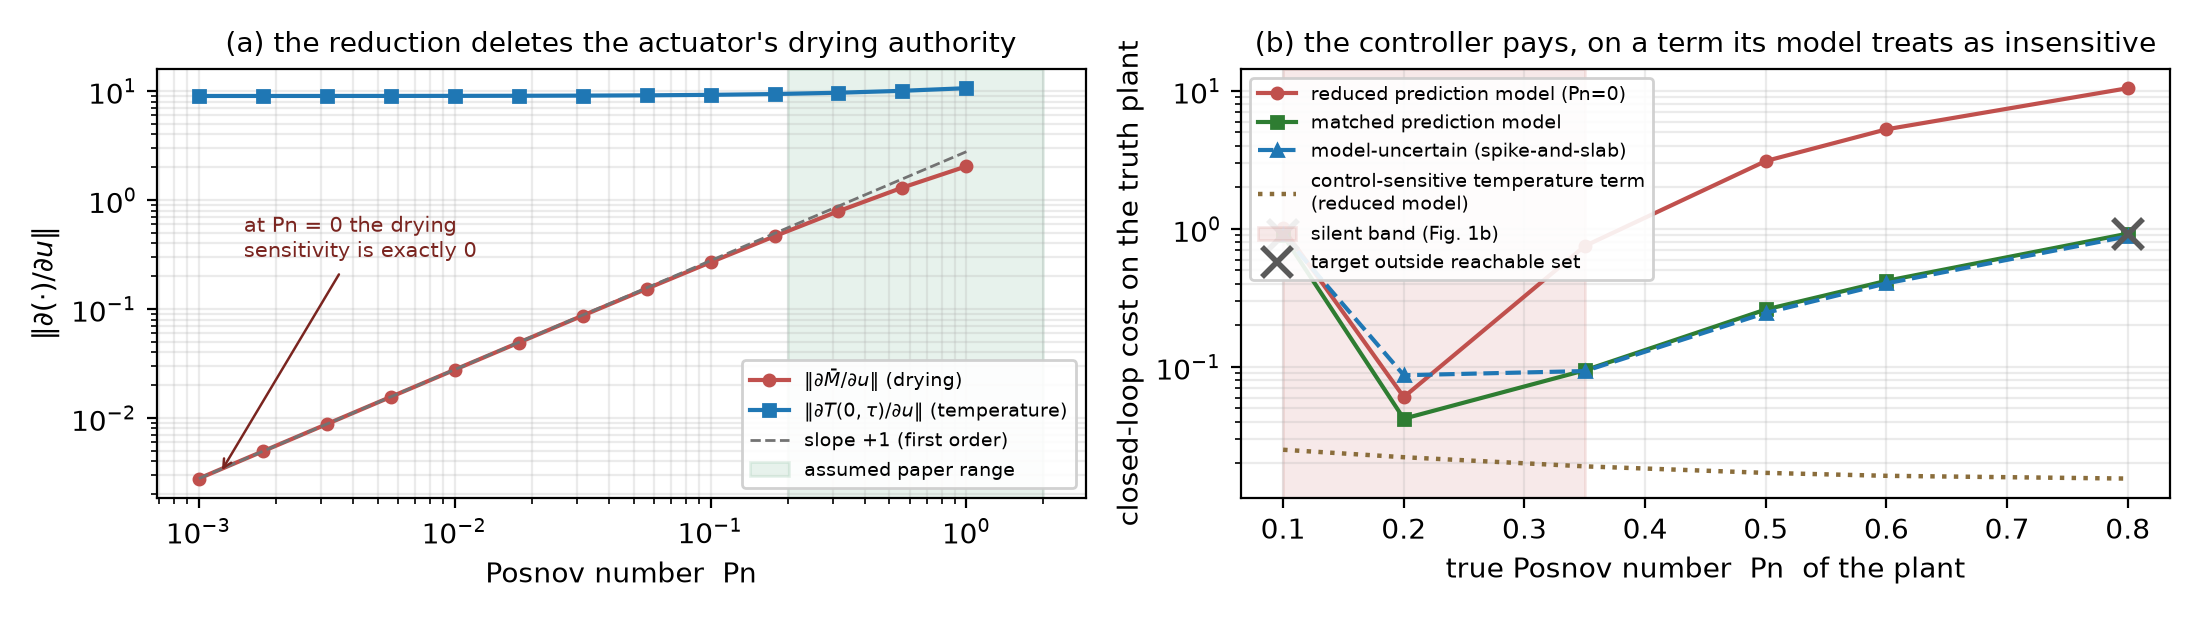
\includegraphics[width=\linewidth]{C_control_structure.png}
\caption{\textbf{(a)} Sensitivity of the drying and temperature observables to the manipulated air
temperature. Exactly zero for moisture at $\mathrm{Pn}{=}0$, $O(\mathrm{Pn})$ thereafter; the
temperature channel is flat and large throughout. \textbf{(b)} Closed-loop cost on the coupled truth
plant. The reduced-model controller's regret grows with the true coupling while the control-sensitive
temperature term under the reduced model (dotted) improves.}
\label{fig:ctrl}
\end{figure}

\paragraph{Reading.} Three points. First, this is a \emph{decision reversal}: at
$\mathrm{Pn}{=}0.6$ the matched controller runs less than half the reduced controller's mean heat
($0.52$ vs $1.09$), because the reduction hides that cooling is the way to dry. Second, the failure is
silent in the same sense as Sec.~5 -- the control-sensitive temperature term under the reduced model
improves monotonically ($0.025\!\to\!0.016$) as its true cost rises by an order of magnitude. Third, $\mathrm{Pn}{=}0.35$
lies inside the silent goodness-of-fit band, so a model that cannot be rejected by fitting the
moisture sensors still costs $8\times$ in closed loop, there commanding a $30\%$ higher mean thermal
input than the matched controller. Model-uncertain control tracks the matched arm
for $\mathrm{Pn}\!\ge\!0.35$, within $\pm5\%$ of it -- comparable rather than better -- while costing
substantially more at $\mathrm{Pn}{=}0.2$, where the coupling is too weak to be worth hedging against.
Every solve uses $4$ multistarts; against a single warm start no closed-loop cost moves by more than
$0.05\%$, so these differences are not local-basin artefacts.

\paragraph{Idealisations.} Full-state feedback (no observer), a solver-in-the-loop shrinking-horizon
NMPC rather than a learned surrogate, and no mapping from dimensionless time to a physical sampling
interval, so no real-time claim is made. These deliberately remove estimator and surrogate quality as
confounds. The coupled plant is bit-identical to the original reduced plant at $\mathrm{Pn}{=}0$ over
$150$ random control steps, and reproduces the benchmark solver to $0.00\mathrm{e}{+}00$ relative
$L_2$ at constant input.

\end{document}
